\documentclass[xcolor=x11names,compress,french]{beamer}
%
%
%%%%%%%%%%%%%%%% General document %%%%%%%%%%%%%%%%
\usepackage{graphicx}
\usepackage{hyperref}
\usepackage[latin1]{inputenc}
\usepackage{color}
\usepackage[french]{babel}
\usepackage{amsmath, amsfonts}
\usepackage{textgreek}
%\usepackage{siunitx}
\usepackage{rotating}
\usepackage{booktabs} % Allows the use of \toprule, \midrule and \bottomrule in tables
%\usepackage{natbib}
%\usepackage{latexsym}
%\usepackage{amssymb}
%
\usepackage{bm}  % bold math
\usepackage{booktabs}  % better tables
\usepackage{multirow}  % combine table rows
\usepackage{makecell}  % arrange content in table cells incl. linebreaks
\usepackage{csquotes}  % quotation/citation commands

%%%%%%%%%%%%%%%% FIGURES %%%%%%%%%%%%%%%%
\usepackage{subfigure}
\usepackage{epsfig} 
\usepackage{epstopdf}
%\usepackage{movie15}
%\usepackage{eurosym}
%\usepackage{gensymb}
%\usepackage{lmodern}
%\usepackage{tabularx}
\usepackage{booktabs}
\usepackage{xcolor}
\usepackage{colortbl}
% Define colors
\definecolor{rowlight}{gray}{0.92}
\definecolor{rowdark}{gray}{0.80}
%\usepackage{float}
%
%%%%%%%%%%%%%%% TIKZ %%%%%%%%%%%%%%%%%%%%
\usepackage{smartdiagram}
\usepackage{metalogo}
%\usepackage{dtklogos}
%
%%%%%%%%%%%%%%%% COLORS %%%%%%%%%%%%%%%%
\definecolor{violet}{rgb}{0.3,0.2,0.6}
\definecolor{violetpale}{rgb}{0.7,0.7,0.8}
\definecolor{marine}{RGB}{25,25,112}
\definecolor{marinepale}{rgb}{0.4,0.4,0.5}
\definecolor{myblue}{rgb}{0.2,0.2,0.7}
\definecolor{mycream}{rgb}{0.9712 0.940 0.807}
%
%
%%%%%%%%%%%%%%%% TEXT BOXES %%%%%%%%%%%%%%%%
\usepackage[absolute,showboxes,overlay]{textpos}
%\TPshowboxestrue % commenter une fois fini
\TPshowboxesfalse % d�commenter pour faire disparaitre les boites
\textblockorigin{10mm}{10mm} % origine des positions
%
%
%%%%%%%%%%%%%%%% BEAMER PACKAGE AND OPTIONS %%%%%%%%%%%%%%%%
%%% Beamer Layout %%%%%%%%%%%%%%%%%%%%%%%%%%%%%%%%%%
%%\usetheme{Madrid}
%%\usetheme{Warsaw}
\usetheme{Frankfurt}
%%\usetheme{Amsterdam}
\setbeamerfont{caption}{size=\scriptsize}
\setbeamertemplate{caption}[numbered]
%%\useoutertheme[subsection=false,shadow]{miniframes}
%%\setbeamertemplate{mini frames}{}
\useinnertheme{default}
\usefonttheme{serif}
\usepackage{palatino}
%%\setbeamertemplate{navigation symbols}{}
\setbeamerfont{frametitle}{size=\small}
\setbeamertemplate{footline}[page number]
%\setbeamercolor*{normal text}{fg=marine,bg=mycream} 
\setbeamercolor*{normal text}{fg=marine,bg=white} 
\setbeamercolor*{alerted text}{fg=red} 
\setbeamercolor*{example text}{fg=black} 
\setbeamercolor*{structure}{fg=marine}  
\setbeamercolor*{palette tertiary}{fg=black,bg=black!10} 
\setbeamercolor*{palette quaternary}{fg=black,bg=black!10} 
\setbeamertemplate{caption}{\raggedright\insertcaption\par}
%%%%%%%%%%%%%%%%%%%%%%%%%%%%%%%%%%%%%%%%%%%%%%%%%%%
\makeatletter
    \newenvironment{withoutheadline}{
        \setbeamertemplate{headline}[default]
        \def\beamer@entrycode{\vspace*{-\headheight}}
    }{}
\setbeamertemplate{mini frames}{}
\setbeamertemplate{headline}{}
\setbeamertemplate{navigation symbols}{}
\definecolor{myred}{rgb}{0.51,0.0,0.0} 
\setbeamercolor{frametitle}{fg=white, bg=myred}
\setbeamercolor{title}{fg=white, bg=myred}
%
%\newlength\leftsidebar
%\newlength\rightsidebar
%\makeatletter
%\setlength\leftsidebar{\beamer@leftsidebar}
%\setlength\rightsidebar{\beamer@rightsidebar}
%%\setbeamercovered{transparent}
%\def\beamertemplatetransparentcoveredmedium{\setbeamercovered{transparent=0.9}}
%\beamertemplatetransparentcoveredmedium
%%
%%\setbeamertemplate{headline}{%
%%\leavevmode%
%%  \hbox{%
%%    \begin{beamercolorbox}[wd=\paperwidth,ht=2.5ex,dp=1.125ex]{palette quaternary}%
%%    \insertsectionnavigationhorizontal{\paperwidth}{}{\hskip0pt plus1filll}
%%    \end{beamercolorbox}%
%%  }
%%}
%%\setbeamertemplate{headline}
%%{%
%%  \leavevmode%
%%  \begin{beamercolorbox}[wd=.3\paperwidth,ht=2.5ex,dp=1.125ex]{section in head/foot}%
%%    \hbox to .3\paperwidth{\hfil\insertsectionhead\hfil}
%%  \end{beamercolorbox}%
%%  \begin{beamercolorbox}[wd=.3\paperwidth,ht=2.5ex,dp=1.125ex]{subsection in head/foot}%
%%    \hbox to .3\paperwidth{\hfil\insertsubsectionhead\hfil}
%%  \end{beamercolorbox}%
%%}
%%\setbeamertemplate{navigation symbols}{} 
%%
%%\setbeamercolor*{lower separation line head}{bg=DeepSkyBlue4} 
%
%
%
%%%%%%%%%%%%%%%% TIKZ %%%%%%%%%%%%%%%%
\usepackage{tikz}
\usetikzlibrary{tikzmark}
\usetikzlibrary{decorations.pathreplacing,calc}
\usetikzlibrary{decorations.fractals}
\usepackage{pgfplots}
\usepackage{pgfplotstable}
%
%



%%%%%%%%%%%%%%%%%%%%%%%%%%%%%%%%%%%%%%%%%%%%%%%%%%%%%%%
%%
%
%\newcommand\MyText[4][0pt]{%
%\begin{tikzpicture}[overlay, remember picture]
%\draw [decoration={brace},decorate,thick]
%   ( $ ({pic cs:#3}|-{pic cs:#2}) + (#1,1.3ex) $ ) --  
%    node[anchor=west,xshift=5pt,text width=5cm] {#4} 
%  ( $ (pic cs:#3) + (#1,0) $ );
%\end{tikzpicture}%
%}

%
%\makeatother
%
%% See if the author has AMS Euler fonts installed: If they have, attempt
%% to use the 'upmath' package to provide upright math.
%%%\usepackage{lipsum}
%%\usepackage{subfigure}
%%\linespread{1.6}
%%\textwidth 14.7 true cm
%%\textheight 21.6 true cm
%
%%\ifCUPmtlplainloaded \else
%%  \checkfont{eurm10}
%%  \iffontfound
%%    \IfFileExists{upmath.sty}
%%      {\typeout{^^JFound AMS Euler Roman fonts on the system,
%%                   using the 'upmath' package.^^J}%
%%       \usepackage{upmath}}
%%      {\typeout{^^JFound AMS Euler Roman fonts on the system, but you
%%                   dont seem to have the}%
%%       \typeout{'upmath' package installed. JFM.cls can take advantage
%%                 of these fonts,^^Jif you use 'upmath' package.^^J}%
%%       \providecommand\upi{\pi}%
%%      }
%%  \else
%%    \providecommand\upi{\pi}%
%%  \fi
%%\fi 
%
%%% See if the author has AMS symbol fonts installed: If they have, attempt
%%% to use the 'amssymb' package to provide the AMS symbol characters.
%
%%\ifCUPmtlplainloaded \else
%%  \checkfont{msam10}
%%  \iffontfound
%%    \IfFileExists{amssymb.sty}
%%      {\typeout{^^JFound AMS Symbol fonts on the system, using the
%%                'amssymb' package.^^J}%
%%       \usepackage{amssymb}%
%%       \let\le=\leqslant  \let\leq=\leqslant
%%       \let\ge=\geqslant  \let\geq=\geqslant
%%      }{}
%%  \fi
%%\fi
%
%%% See if the author has the AMS 'amsbsy' package installed: If they have,
%%% use it to provide better bold math support (with \boldsymbol).
%
%%\ifCUPmtlplainloaded \else
%%  \IfFileExists{amsbsy.sty}
%%    {\typeout{^^JFound the 'amsbsy' package on the system, using it.^^J}%
%%     \usepackage{amsbsy}}
%%    {\providecommand\boldsymbol[1]{\mbox{\boldmath $##1$}}}
%%\fi
%
%
%%%% Example macros (some are not used in this sample file) %%%
%
%%Comments
%\def\NOTE#1{{\textcolor{red}{\bf [#1]}}}  % note
%\def\ADD#1{{\textcolor{blue}{\bf #1}}}    % question
%
%% For units of measure
%\newcommand\dynpercm{\nobreak\mbox{$\;$dyn\,cm$^{-1}$}}
%\newcommand\cmpermin{\nobreak\mbox{$\;$cm\,min$^{-1}$}}
%
%% Various bold symbols
%\providecommand\bnabla{\boldsymbol{\nabla}}
%\providecommand\bcdot{\boldsymbol{\cdot}}
%\newcommand\biS{\boldsymbol{S}}
%\newcommand\etb{\boldsymbol{\eta}}
%
%% For multiletter symbols
%\newcommand\Real{\mbox{Re}} % cf plain TeX's \Re and Reynolds number
%\newcommand\Imag{\mbox{Im}} % cf plain TeX's \Im
%\newcommand\Rey{\mbox{\textit{Re}}}  % Reynolds number
%\newcommand\Pran{\mbox{\textit{Pr}}} % Prandtl number, cf TeX's \Pr product
%\newcommand\Pen{\mbox{\textit{Pe}}}  % Peclet number
%\newcommand\Ai{\mbox{Ai}}            % Airy function
%\newcommand\Bi{\mbox{Bi}}            % Airy function
%
%% For sans serif characters:
%% The following macros are setup in JFM.cls for sans-serif fonts in text
%% and math.  If you use these macros in your article, the required fonts
%% will be substitued when you article is typeset by the typesetter.
%%
%% \textsfi, \mathsfi   : sans-serif slanted
%% \textsfb, \mathsfb   : sans-serif bold
%% \textsfbi, \mathsfbi : sans-serif bold slanted (doesnt exist in CM fonts)
%%
%% For san-serif roman use \textsf and \mathsf as normal.
%%
%\newcommand\ssC{\mathsf{C}}    % for sans serif C
%\newcommand\sfsP{\mathsfi{P}}  % for sans serif sloping P
%\newcommand\slsQ{\mathsfbi{Q}} % for sans serif bold-sloping Q
%
%% Hat position
%\newcommand\hatp{\skew3\hat{p}}      % p with hat
%\newcommand\hatR{\skew3\hat{R}}      % R with hat
%\newcommand\hatRR{\skew3\hat{\hatR}} % R with 2 hats
%\newcommand\doubletildesigma{\skew2\tilde{\skew2\tilde{\Sigma}}}
%%       italic Sigma with double tilde
%
%% array strut to make delimiters come out right size both ends
%\newsavebox{\astrutbox}
%\sbox{\astrutbox}{\rule[-5pt]{0pt}{20pt}}
%\newcommand{\astrut}{\usebox{\astrutbox}}
%
%\newcommand\GaPQ{\ensuremath{G_a(P,Q)}}
%\newcommand\GsPQ{\ensuremath{G_s(P,Q)}}
%\newcommand\p{\ensuremath{\partial}}
%\newcommand\tti{\ensuremath{\rightarrow\infty}}
%\newcommand\kgd{\ensuremath{k\gamma d}}
%\newcommand\shalf{\ensuremath{{\scriptstyle\frac{1}{2}}}}
%\newcommand\sh{\ensuremath{^{\shalf}}}
%\newcommand\smh{\ensuremath{^{-\shalf}}}
%\newcommand\squart{\ensuremath{{\textstyle\frac{1}{4}}}}
%\newcommand\thalf{\ensuremath{{\textstyle\frac{1}{2}}}}
%\newcommand\Gat{\ensuremath{\widetilde{G_a}}}
%\newcommand\ttz{\ensuremath{\rightarrow 0}}
%\newcommand\ndq{\ensuremath{\frac{\mbox{$\partial$}}{\mbox{$\partial$} n_q}}}
%\newcommand\sumjm{\ensuremath{\sum_{j=1}^{M}}}
%\newcommand\pvi{\ensuremath{\int_0^{\infty}%
%  \mskip \ifCUPmtlplainloaded -30mu\else -33mu\fi -\quad}}
%
%\newcommand\etal{\mbox{\textit{et al.}}}
%\newcommand\etc{etc.\ }
%\newcommand\eg{e.g.\ }
%
%\newcommand\VA{\ensuremath{{\cal{V}}}}
%\newcommand\AV{\ensuremath{{\cal{A}}}}
%
%
%
%% Figures..
%\pgfplotsset{filter discard warning=false} % Emp?che l'affichage des warning lorsqu'un NaN est pr?sent dans le csv
\usepackage{textcomp}

\usepackage[thicklines]{cancel}
\newcommand\Ccancel[2][black]{\renewcommand\CancelColor{\color{#1}}\xcancel{#2}}
%
\definecolor{myblue}{rgb}{0.0, 0.0, 0.86}
\definecolor{myBlue}{rgb}{0.0, 0.0, 0.86}
\definecolor{mygreen}{rgb}{0, 0.5, 0}
\definecolor{myred}{rgb}{0.41, 0, 0}
\definecolor{airforceblue}{rgb}{0.36, 0.54, 0.66}

%% \definecolor{myred}{RGB}{105,0,0} 
%\setbeamercolor{block title}{bg=myred,fg=white}
%
\graphicspath{{./images/}{figures/},{./01_IP_intro/},{./02_IP_results/},{./03_Tigrou/}}
%
%
\newcommand{\dless}{\mathrm}  % style of dimensionless numbers
\renewcommand{\Re}{\dless{Re}}  % Reynolds number
\newcommand{\Ar}{\dless{Ar}}  % Archimedes number
\newcommand{\Ga}{\dless{Ga}}  % Galileo number
%
%
\usepackage[per-mode=symbol-or-fraction, separate-uncertainty]
{siunitx}  % typeset numbers & units
\DeclareSIUnit{\pixel}{px}  % custom pixel unit
%
%
\begin{document}
%\addtocounter{framenumber}{-6}
%
%
%%%%%%%%%%%%%%%%%%%%%%%%%%%%%%%%%%%%%%%%%%%%%%%%%%%%%%%%%%%%%%%%%%%%%%%%%%
% PAGE DE TITRE
%%%%%%%%%%%%%%%%%%%%%%%%%%%%%%%%%%%%%%%%%%%%%%%%%%%%%%%%%%%%%%%%%%%%%%%%%%
%
\begin{withoutheadline}
\begin{frame}
%\titlegraphic{\includegraphics[width=0.8\textwidth]{SpotHDR.eps}}

\title{Inertial Particles and Turbulence}
%
\author{Romain Monchaux\\[6pt]}
%
\institute{Unit� de M�canique\\[4pt]
ENSTA - Institut Polytechnique de Paris, Palaiseau, France}
\date{}
\titlepage
\vspace{-27pt}
\begin{center}
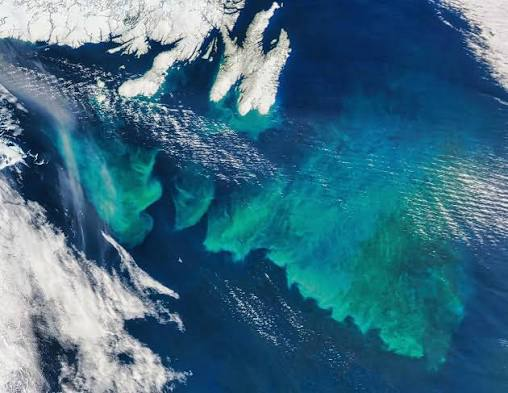
\includegraphics[width=.40\textwidth]{images.jpeg}\\[10pt]
\footnotesize{November 25$^{th}$ 2026 - Chatou}
\end{center}
\end{frame}
\end{withoutheadline}
%
%
%%%%%%%%%%%%%%%%%%%%%%%%%%%%%%%%%%%%%%%%%%%%%%%%%%%%%%%%%%%%%%%%%%%%%%%%%%
% INTRO 
\section{Introduction}
\begin{frame}
\frametitle{Inertial particles and turbulence}
	% Applications
%    \begin{textblock*}{90mm}[0,0](-5mm,-2mm)
%    \textcolor{myred}{\textbf{Many fields of application}}
%    \begin{itemize}
%        \item \textbf{Natural} : plankton, marine snow, rain, pollutants
%        \item \textbf{Industrial} : chemical reactors, combustion chambers
%    \end{itemize}
%    \end{textblock*}
    
\begin{textblock*}{30mm}[0,0](0mm,2mm)
	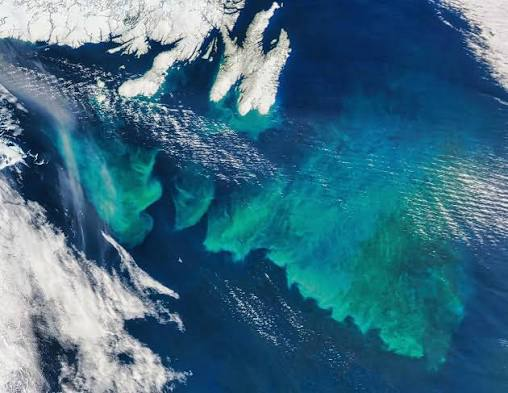
\includegraphics[width = \textwidth]{images.jpeg}
\end{textblock*}
\begin{textblock*}{30mm}[0,0](-5mm,30mm)
	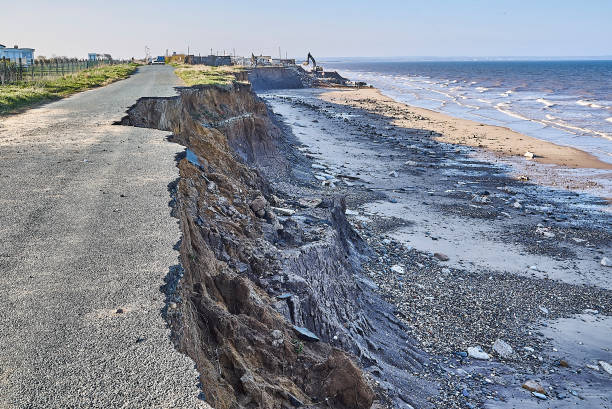
\includegraphics[width = \textwidth]{gravity_erosion.jpg}
\end{textblock*}
\begin{textblock*}{70mm}[0,0](0mm,55mm)
	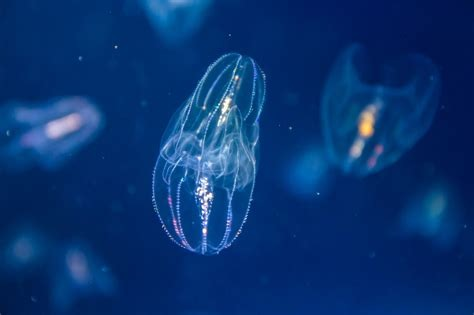
\includegraphics[clip,trim=0 0 0 0,width = .45\textwidth]{plankton.jpg}
\end{textblock*}

\begin{textblock*}{30mm}[0,0](42mm,-1mm)
	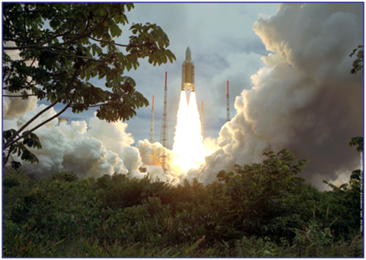
\includegraphics[width = \textwidth]{Fusee.png}
\end{textblock*}
\begin{textblock*}{70mm}[0,0](37mm,24mm)
	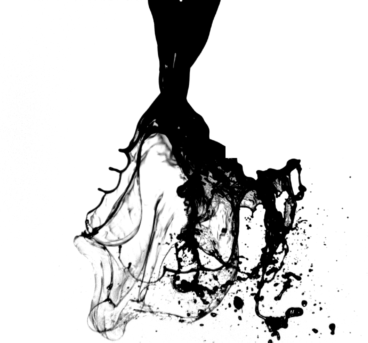
\includegraphics[clip,trim=0 0 0 0,width = .5\textwidth]{150SLPM_nice.png}
\end{textblock*}
\begin{textblock*}{40mm}[0,0](39mm,62mm)
	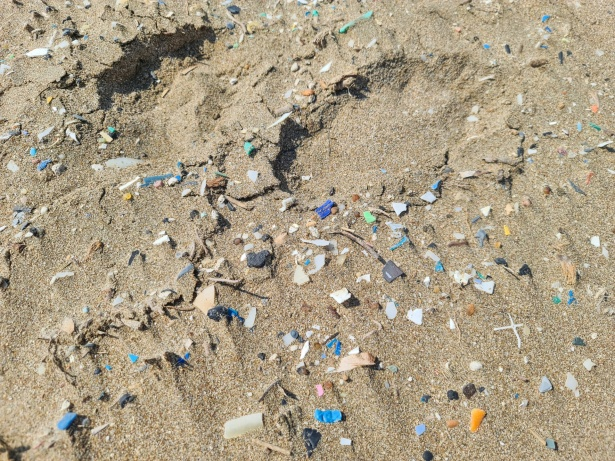
\includegraphics[clip, trim=0 30 0 150 , width = \textwidth]{microplastics-on-the-beach-1662635283OyR.jpg}
\end{textblock*}


\begin{textblock*}{30mm}[0,0](83mm,0mm)
	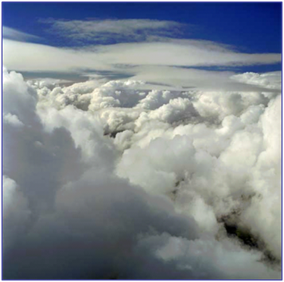
\includegraphics[width = \textwidth]{Nuages.png}
\end{textblock*}
\begin{textblock*}{30mm}[0,0](83mm,35mm)
	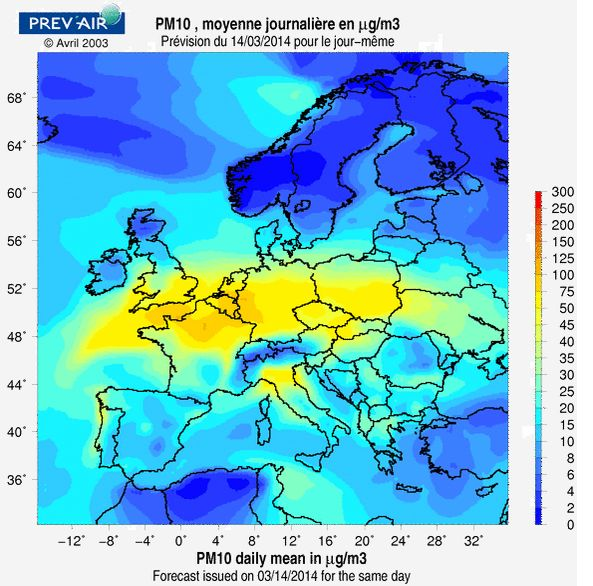
\includegraphics[clip,trim=30 45 58 55,width = \textwidth]{Carte_PM10_Europe_20140314.JPG}
\end{textblock*}
%	{%
%		\setlength{\fboxsep}{0pt}%
%		\setlength{\fboxrule}{1pt}%
%		\fbox{\includegraphics[options]{image}}%
%	}%


\end{frame}
%%%%%%%%%%%%%%%%%%%%%%%%%%%%%%%%%%%%%%%%%%%%%%%%%%%%%%%%%%%%%%%%%%%%%%%%%%
% PART: SLIDE n°3
\frame{
\frametitle{Tracers \textit{vs} Inertial Particles}
\begin{textblock*}{45mm}[0,0](-4mm,0mm)
   	\footnotesize{Tracers behave as fluid particles}\\[2pt]
	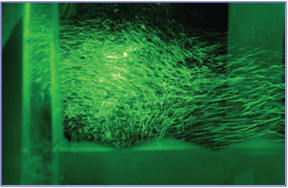
\includegraphics[width=\textwidth]{tracer.png}
\end{textblock*}
\begin{textblock*}{30mm}[0,0](5mm,30mm)
	\small{\textcolor{white}{PIV, LDV, PTV}}
\end{textblock*}

\begin{textblock*}{60mm}[0,0](51mm,0mm)
	\footnotesize{Inertial particles do not follow the flow}\\[2pt]
	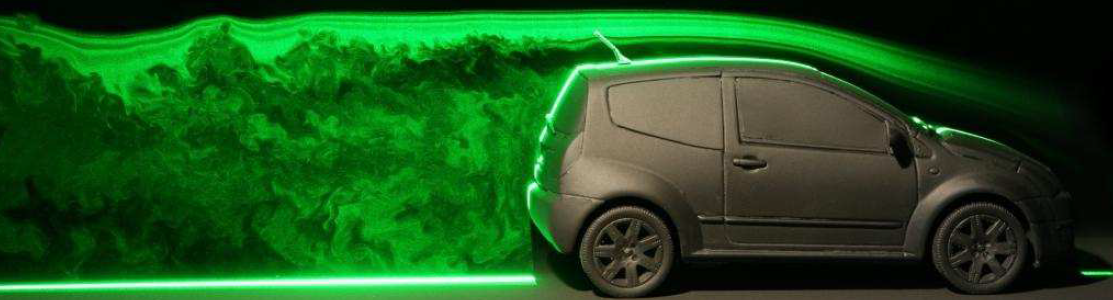
\includegraphics[clip,trim=90 0 70 0,height=22mm]{sillage_voiture.png}
\end{textblock*}
\begin{textblock*}{80mm}[0,0](82mm,28mm)
	\tiny{Grandemange et al, ENSTA 2016}
\end{textblock*}
%
\begin{textblock*}{30mm}[0,0](0mm,40mm)
\onslide<2->{
	\footnotesize{Cluster formation}\\[2pt]
	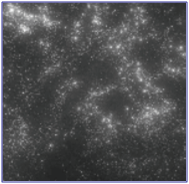
\includegraphics[width=30mm]{inertial.png}
}
\end{textblock*}
\begin{textblock*}{30mm}[0,0](4mm,74mm)
\onslide<2->{
	\tiny{Wood \textit{et al.},	\textit{IJMF}, 31, \textbf{2005}}
}
\end{textblock*}
%
\begin{textblock*}{30mm}[0,0](40mm,40mm)
\onslide<3->{
	\footnotesize{Settling alteration}\\[2pt]
	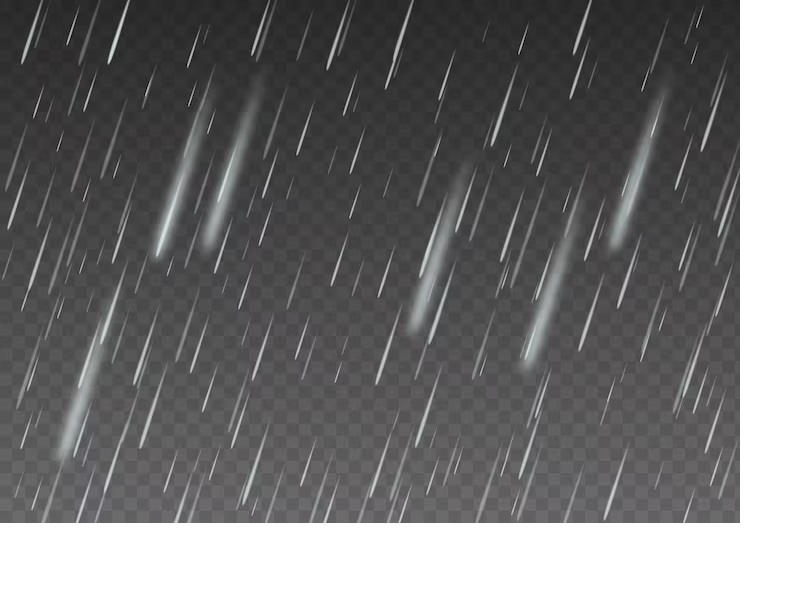
\includegraphics[clip,trim=60 0 60 0,width=30mm]{rain_enhance.jpg}
}
\end{textblock*}
\begin{textblock*}{30mm}[0,0](55mm,70mm)
\onslide<3->{
	\tiny{Artist view}
}
\end{textblock*}
%
\begin{textblock*}{30mm}[0,0](80mm,40mm)
\onslide<4->{
	\footnotesize{Collision alteration}\\[2pt]
	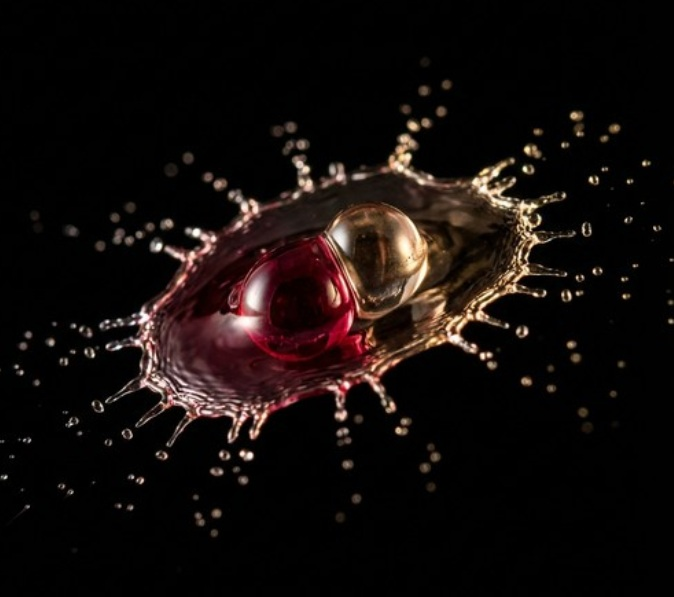
\includegraphics[width=30mm]{collision.jpg}
}
\end{textblock*}
\begin{textblock*}{30mm}[0,0](95mm,71mm)
\onslide<4->{
	\tiny{Artist view}
}
\end{textblock*}
%
\begin{textblock*}{30mm}[0,0](52mm,77mm)
\onslide<5->{
	\footnotesize{Flow modulation, Dispersion\ldots}
}
\end{textblock*}

%
}
\begin{frame}
\frametitle{Inertial particles and turbulence}
	% Applications
%    \begin{textblock*}{90mm}[0,0](-5mm,-2mm)
%    \textcolor{myred}{\textbf{Many fields of application}}
%    \begin{itemize}
%        \item \textbf{Natural} : plankton, marine snow, rain, pollutants
%        \item \textbf{Industrial} : chemical reactors, combustion chambers
%    \end{itemize}
%    \end{textblock*}
    
\begin{textblock*}{30mm}[0,0](0mm,2mm)
	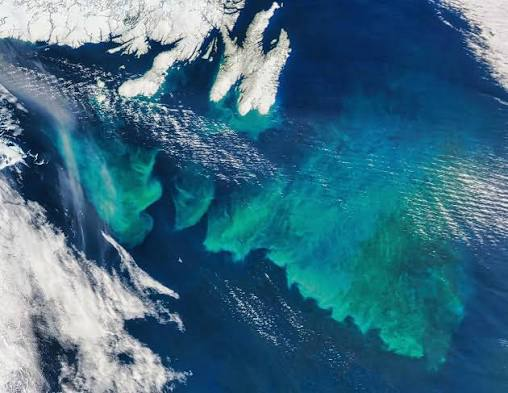
\includegraphics[width = \textwidth]{images.jpeg}
\end{textblock*}

\begin{textblock*}{70mm}[0,0](0mm,45mm)
	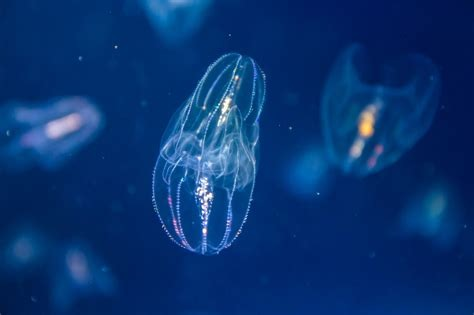
\includegraphics[clip,trim=0 0 0 0,width = .45\textwidth]{plankton.jpg}\\[2pt]
	\footnotesize{Increase meeting\\probabilities}
\end{textblock*}

\begin{textblock*}{30mm}[0,0](42mm,-1mm)

\end{textblock*}
\begin{textblock*}{40mm}[0,0](40mm,14mm)
\textcolor{myred}{{\textbf{Cluster formation}}}\\[4pt]
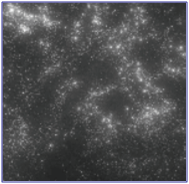
\includegraphics[width=30mm]{inertial.png}
\end{textblock*}
\begin{textblock*}{40mm}[0,0](39mm,62mm)
	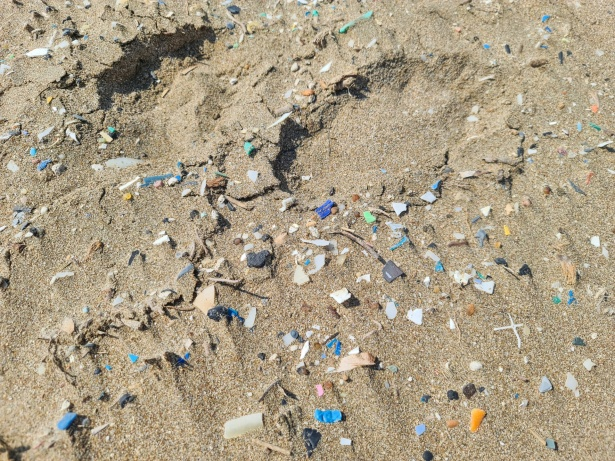
\includegraphics[clip, trim=0 30 0 150 , width = \textwidth]{microplastics-on-the-beach-1662635283OyR.jpg}
\end{textblock*}

\begin{textblock*}{30mm}[0,0](83mm,0mm)
	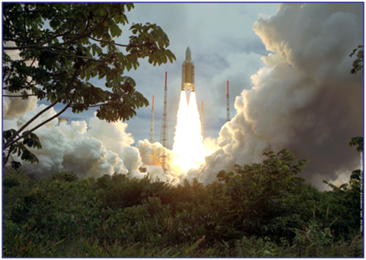
\includegraphics[width = \textwidth]{Fusee.png}\\[2pt]
	\footnotesize{Stoichiometric proportion}
\end{textblock*}
\begin{textblock*}{30mm}[0,0](83mm,35mm)
	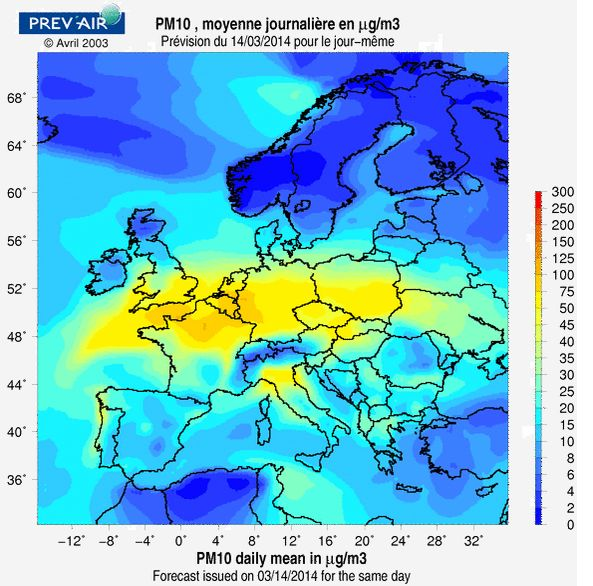
\includegraphics[clip,trim=30 45 58 55,width = \textwidth]{Carte_PM10_Europe_20140314.JPG}\\[2pt]
	\footnotesize{Sanitary thresholds}
\end{textblock*}
%	{%
%		\setlength{\fboxsep}{0pt}%
%		\setlength{\fboxrule}{1pt}%
%		\fbox{\includegraphics[options]{image}}%
%	}%


\end{frame}
\begin{frame}
\frametitle{Inertial particles and turbulence}
	% Applications
%    \begin{textblock*}{90mm}[0,0](-5mm,-2mm)
%    \textcolor{myred}{\textbf{Many fields of application}}
%    \begin{itemize}
%        \item \textbf{Natural} : plankton, marine snow, rain, pollutants
%        \item \textbf{Industrial} : chemical reactors, combustion chambers
%    \end{itemize}
%    \end{textblock*}
    
\begin{textblock*}{30mm}[0,0](0mm,2mm)
	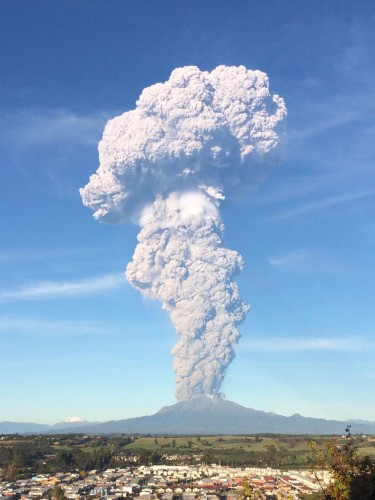
\includegraphics[width = \textwidth]{volcano.jpg}
\end{textblock*}
\begin{textblock*}{45mm}[0,0](0mm,45mm)
{\footnotesize Aerosol and climate forcing\\
Aviation safety\\
}\end{textblock*}

\begin{textblock*}{35mm}[0,0](42mm,-1mm)
	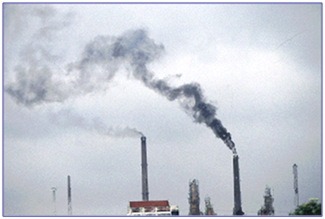
\includegraphics[width = \textwidth]{Cheminees.png}
\end{textblock*}
\begin{textblock*}{35mm}[0,0](40mm,30mm)
	\centering
\textcolor{myred}{{\textbf{Settling alteration\\-\\Dispersion}}}
\end{textblock*}
\begin{textblock*}{30mm}[0,0](5mm,55mm)
	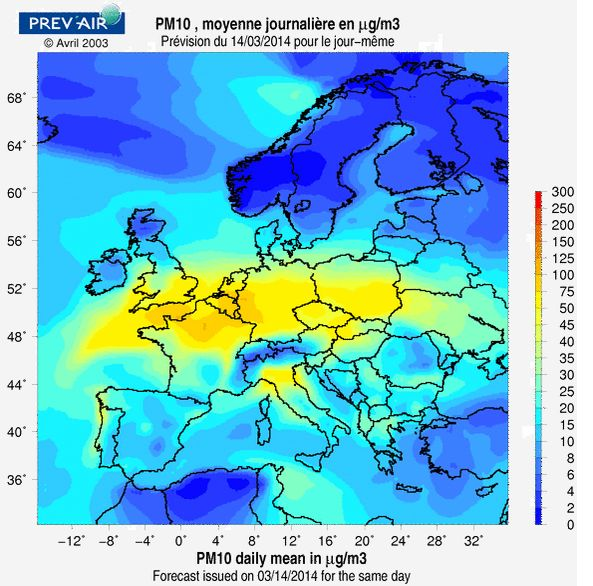
\includegraphics[clip,trim=30 45 58 55,width = \textwidth]{Carte_PM10_Europe_20140314.JPG}
\end{textblock*}


\begin{textblock*}{30mm}[0,0](83mm,0mm)
	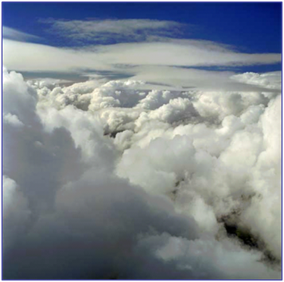
\includegraphics[width = \textwidth]{Nuages.png}\\
	\footnotesize{Rain formation alteration}
\end{textblock*}
\begin{textblock*}{30mm}[0,0](83mm,43mm)
	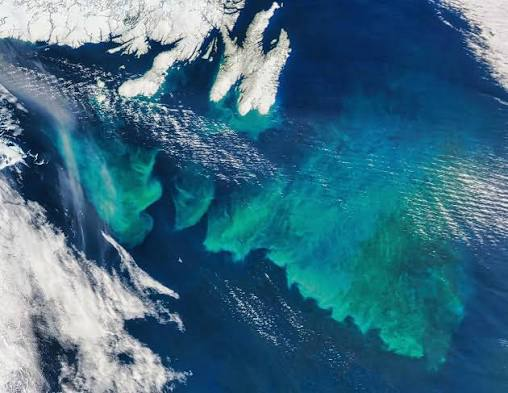
\includegraphics[width = \textwidth]{images.jpeg}
\end{textblock*}
\begin{textblock*}{34mm}[0,0](42mm,50mm)
	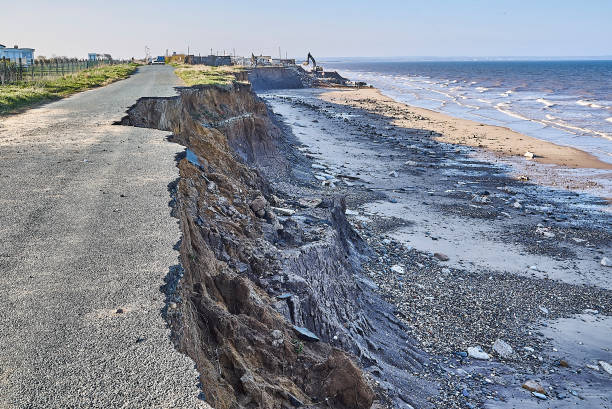
\includegraphics[width = \textwidth]{gravity_erosion.jpg}
\end{textblock*}

\begin{textblock*}{55mm}[0,0](60mm,75mm)
{\footnotesize Marine snow : carbon pump\\
	Estuaries dynamics}\\
\end{textblock*}


%	{%
%		\setlength{\fboxsep}{0pt}%
%		\setlength{\fboxrule}{1pt}%
%		\fbox{\includegraphics[options]{image}}%
%	}%


\end{frame}
\frame{
\frametitle{Inertial Particles and Turbulence}

\begin{textblock*}{55mm}[0,0](0mm,0mm)
	\centering
	\only<1-2>{
		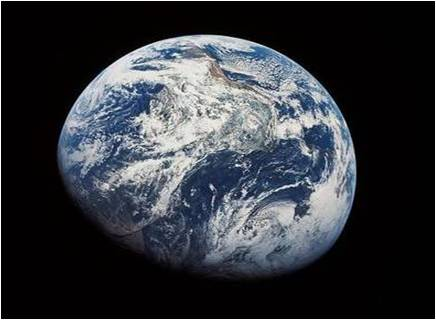
\includegraphics[height=40mm]{atm.jpg}
	}
\end{textblock*}

\begin{textblock*}{55mm}[0,0](60mm,0mm)
	\centering
	\only<1-2>{
		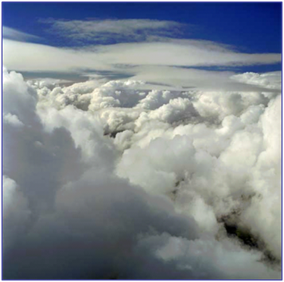
\includegraphics[height=40mm]{Nuages.png}
	}
\end{textblock*}

\begin{textblock*}{55mm}[0,0](25mm,44mm)
	\centering
	\only<2>{
		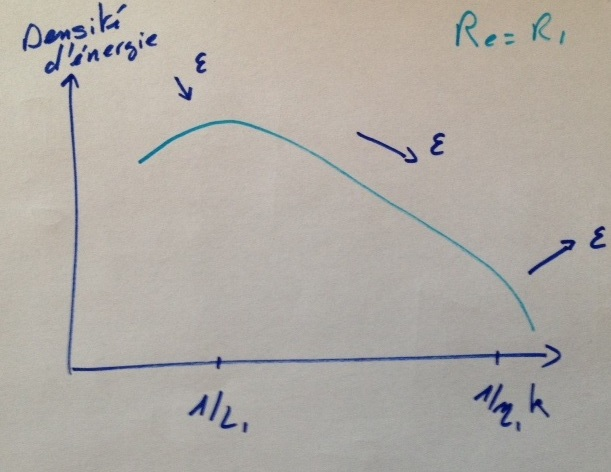
\includegraphics[width=\textwidth]{specTBL1.JPG}
	}
\end{textblock*}



\begin{textblock*}{55mm}[0,0](-5mm,0mm)
	\centering
	\only<3-5,8>{	
%		Density: $\rho_p\neq \rho_f$\\[6pt]
		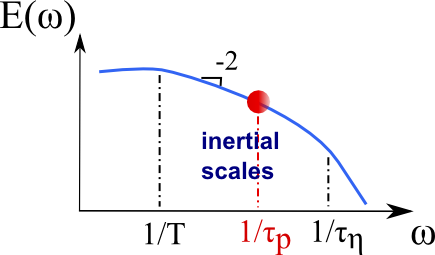
\includegraphics[width=\textwidth]{pseudoSpectre2.png}
	}
\end{textblock*}


\begin{textblock*}{55mm}[0,0](65mm,3mm)
	\only<5>{\textbf{\textcolor{myred}{Response time:}}	\\[4pt]
{\small	Stokes drag: $\tau_p = \rho_p d_p^2 / 18\mu$\\[2pt]
	Non linear drag: $\tau_p^{eff}(|\mathbf{w}|)$\\[2pt]
	Added mass: $\tau_p^{am}$\\[2pt]
	Basset history: \ldots
}}
\end{textblock*}
%
%
\begin{textblock*}{55mm}[0,0](-5mm,0mm)
	\centering
	\only<6-7>{	
		%		Density: $\rho_p\neq \rho_f$\\[6pt]
		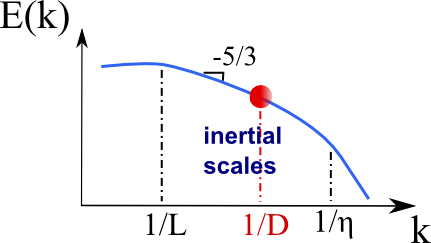
\includegraphics[width=\textwidth]{pseudoSpectre1.png}
	}
\end{textblock*}


\begin{textblock*}{55mm}[0,0](55mm,0mm)
	\centering
	\only<8->{	
		%		Size: $\eta < D < L$\\[6pt]
		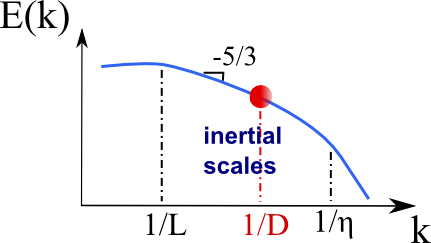
\includegraphics[width=\textwidth]{pseudoSpectre1.png}}
\end{textblock*}
%
%
\begin{textblock*}{90mm}[0,0](-5mm,37mm)
	\only<7>
	{\small{\textbf{Finite size effects:}}
	\begin{itemize}
		\item Fax\'en corrections ($d_p\leq \eta$)
		\item Filtering of small scales, integration over particle size
		\item Anisotropy
		\begin{itemize}
		\item Rotation / tumbling inertia
	\item Porosity and roughness
		\end{itemize}
		\item \ldots
	\end{itemize}
	}
\end{textblock*}
%
\begin{textblock*}{90mm}[0,0](-5mm,34mm)
	\only<8>{
{\footnotesize
\renewcommand{\arraystretch}{1.4}
\begin{tabular}{lll}
	\textbf{Source} & \textbf{Timescale} & \textbf{Relevant when} \\
	\midrule
	\rowcolor{rowlight}
	Stokes drag & $\tau_p = \rho_p d_p^2 / 18\mu$ & Always, baseline \\
	\rowcolor{rowdark}
	Nonlinear drag & $\tau_p^{eff}(|\mathbf{w}|)$ & $Re_p \gtrsim 1$ \\
	\rowcolor{rowlight}
	Added mass & $\tau_p^{am}$ & $\rho_p / \rho_f \sim \mathcal{O}(1)$ \\
	\rowcolor{rowdark}
	Basset history &complex kernel & Unsteady $\mathbf{w}$, $\rho_p / \rho_f$ moderate \\
	\rowcolor{rowlight}
	Orientational inertia & $\tau_{rot}$ & Non-spherical particles \\
	\rowcolor{rowdark}
	Finite size filtering & $d_p / \eta$ & $d_p \gtrsim \eta$ \\
	\rowcolor{rowlight}
	Porosity/permeability & Internal flow timescale & Aggregates, flocs \\
	\bottomrule
\end{tabular}
}
	}
\end{textblock*}
%
\begin{textblock*}{90mm}[0,0](-5mm,37mm)
	\only<4-5>
	{\small{\textbf{Model point particle equation:}}
		\scriptsize{
			\begin{eqnarray*}
				\rho_p\frac{\partial v_i}{\partial t}
				&=&
				% gravity
				\overbrace{
					(\rho_p-\rho_f)g_i}
				^{\mathrm{gravity}}
				% undisturbed flow
				+ \overbrace{
					\frac{\partial \tau _{ij}}{\partial x_j}	
					-\frac{\partial p}{\partial x_i}
				}
				^{\mathrm{undisturbed\ flow}}
				% steady state drag
				+\overbrace{
					\frac{9}{2}\frac{\mu}{r_p^2}\biggl (
					(u_i-v_i) + \frac{r_p^2}{6} {\nabla} ^2u_i
					\biggr)
				}
				^{\mathrm{steady\ state\ drag}}\\
				&&+
				% virtual or apparent mass term
				\overbrace{
					\frac{1}{2}\rho_f \frac{d}{dt}\biggl (
					(u_i-v_i)+ \frac{r_p^2}{10}\nabla^2u_i
					\biggr)
				}
				^{\mathrm{virtual\ or\ apparent\ mass\ term}}
				+
				% Basset history term
				\overbrace{
					\frac{24 \mu}{r_p}\int_0^t\frac{d/dt\biggl(
						u_i-v_i+r_p^2/6\nabla^2u_i
						\biggr)}
					{\pi \nu (t-\tau)^{1/2}}d\tau
				}
				^{\mathrm{Basset\ history\ term}}
			\end{eqnarray*}
	}}
\end{textblock*}
\begin{textblock*}{30mm}[0,0](77mm,76mm)
	\only<4-5>{\tiny{\begin{flushright}
				Maxey \& Riley, \textit{POF}, 26, \textbf{1983}\\
				Gattignol, \textit{JMTA}, 2, \textbf{1983} 
			\end{flushright}
	}}
\end{textblock*}  

}

\frame{
\frametitle{Control parameters}
%
\begin{textblock*}{90mm}[0,0](-10mm,0mm)
\begin{tabular}{ccccc}
\scriptsize{Reynolds number}&
\scriptsize{Stokes number}&
\scriptsize{Rouse number}&
\scriptsize{Density ratio}&
\scriptsize{Loading}\\
\footnotesize{$\bold{R_{\lambda}} = \frac{\textcolor{myblue}{u'} \textcolor{myblue}{\lambda}}{\textcolor{myblue}{\nu}};$}&
\footnotesize{$\bold{St} =  \tiny{\frac{2}{9}} \left( \frac{\textcolor{red}{r_p}}{\textcolor{myblue}{\eta}}\right)^2 \left( \frac{\textcolor{red}{\rho_p}}{\textcolor{myblue}{\rho_f}}-1\right);$}&
\footnotesize{$\bold{R} = \frac{\textcolor{mygreen}{v_t}}{\textcolor{myblue}{u'}}; $}&
\footnotesize{${\Gamma} = \frac{\textcolor{red}{\rho _p} }{\textcolor{myblue}{\rho _f}};$}&
%\footnotesize{$\bold{Gamma} = \frac{\textcolor{red}{\rho _p}}/ \textcolor{myblue}{\rho _f}};$}&
\footnotesize{${\Phi _v}.$}\\[8pt]
\scriptsize{\textbf{Turbulence}}&
\scriptsize{\textbf{Inertia}}&
\scriptsize{\textbf{Gravity}}&
\scriptsize{\textbf{Density}}&
\scriptsize{\hspace{-2mm}\textbf{Retroaction}}\\[8pt]
\scriptsize{$10-10^4$}&
\scriptsize{$10^{-5}-10^2$}&
\scriptsize{$0-10$}&
\scriptsize{$10^{-4}-10^3$}&
\scriptsize{\hspace{-3mm}$10^{-6}-10^{-1}$}
\end{tabular}
\end{textblock*}
%\scriptsize{}&
%

\begin{textblock*}{75mm}[0,0](40mm,25mm)
\onslide*<2->{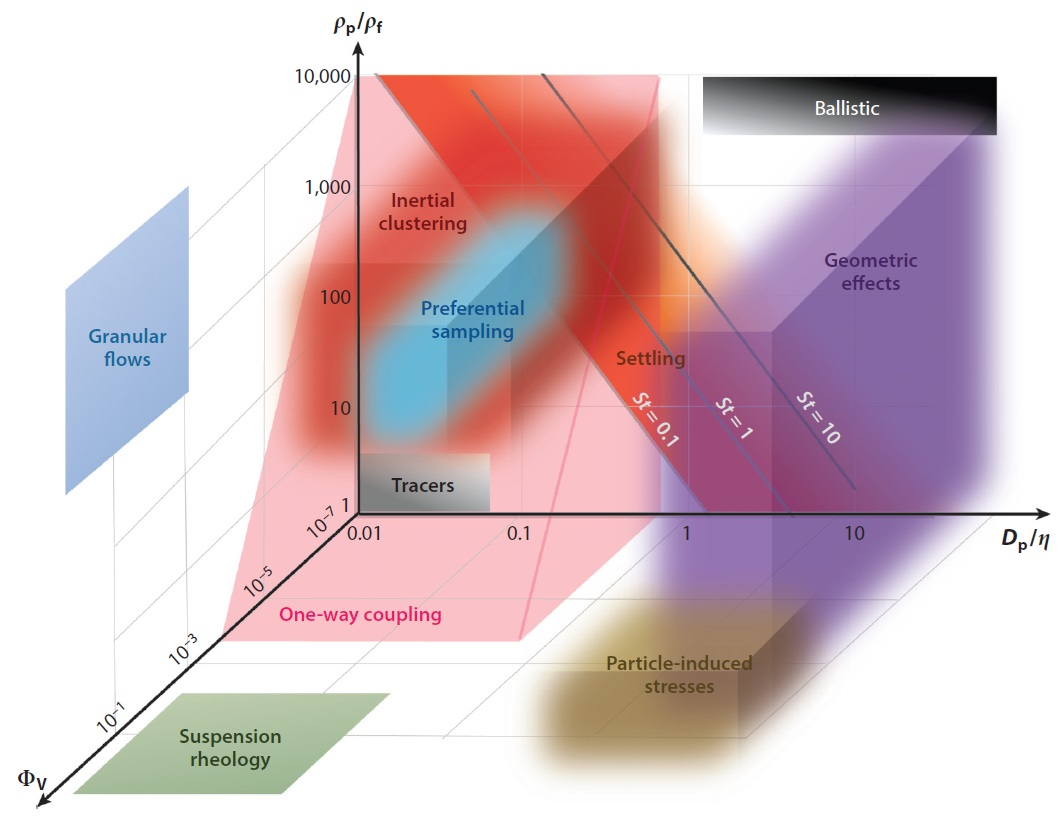
\includegraphics[width = \textwidth]{phase_space_colletti.jpg}}
\end{textblock*}
\begin{textblock*}{20mm}[0,0](95mm,73mm)
{\tiny
\begin{flushright}
\onslide*<2->{	Brandt \& Coletti, \textit{Annual Review}, \textbf{2022}}
\end{flushright}
}
\end{textblock*}
%

\begin{textblock*}{90mm}[0,0](-5mm,32mm)
	{\footnotesize
		\begin{itemize}
			\item Particle Reynolds number
			\item Galileo number
			\item Aspect ratio
			\item Deformability
			\item \ldots
	\end{itemize}}
\end{textblock*}

\begin{textblock*}{50mm}[0,0](-5mm,62mm)
\onslide*<3>{
{\small 
\textcolor{myred}{
\textbf{
Intertwined parameters\\[3pt]}
$\implies$ complementary simulations and experiments}
}}
\end{textblock*}
%
%
}



\frame{
\frametitle{Simulations}
\begin{textblock*}{90mm}[0,0](-5mm,-2mm)
	\textcolor{myred}{\textbf{Point particle approaches}}
\end{textblock*}

\begin{textblock*}{125mm}[0,0](-8mm,4mm)
%\small{\textbf{Fluid equations:}}
%	\scriptsize{
%	\begin{eqnarray*}
%		\frac{\partial {u_i}}{\partial {t}}+\frac{\partial {u_ju_i}}{\partial {x_j}}
%		&=&
%		-\frac{1}{\rho}\frac{\partial {p}}{\partial {x_i}} 
%		+\nu\frac{\partial^2 {u_i}}{\partial {x_j}\partial {x_j}} +{f_i} -{f_i^{(p)}}
%		+{F_{i}}^0,\\
%		\frac{\partial u_i}{\partial x_i}&=&0.
%		\label{navier-stokes}
%	\end{eqnarray*}
%}
\only<1>
{\small{\textbf{Particle equation (Maxey-Riley-Gattignol):}}
\scriptsize{
\begin{eqnarray*}
\rho_p\frac{\partial v_i}{\partial t}
&=&
% gravity
\overbrace{
(\rho_p-\rho_f)g_i}
^{\mathrm{gravity}}
% undisturbed flow
+ \overbrace{
\frac{\partial \tau _{ij}}{\partial x_j}	
-\frac{\partial p}{\partial x_i}
}
^{\mathrm{undisturbed\ flow}}
% steady state drag
+\overbrace{
	\frac{9}{2}\frac{\mu \ f_D}{r_p^2}\biggl (
	(u_i-v_i) + \frac{r_p^2}{6} {\nabla} ^2u_i
	\biggr)
}
^{\mathrm{steady\ state\ drag}}\\
&&+
% virtual or apparent mass term
\overbrace{
	\frac{1}{2}\rho_f \frac{d}{dt}\biggl (
	(u_i-v_i)+ \frac{r_p^2}{10}\nabla^2u_i
	\biggr)
}
^{\mathrm{virtual\ or\ apparent\ mass\ term}}
+
% Basset history term
\overbrace{
	\frac{24 \mu}{r_p}\int_0^t\frac{d/dt\biggl(
		u_i-v_i+r_p^2/6\nabla^2u_i
		\biggr)}
	{\pi \nu (t-\tau)^{1/2}}d\tau
}
^{\mathrm{Basset\ history\ term}}
\end{eqnarray*}
}}
%
%
\only<2>
{\small{\textbf{Particle equation:}}
	\scriptsize{
		\begin{eqnarray*}
			\rho_p\frac{\partial v_i}{\partial t}
			&=&
			% gravity
			\overbrace{
				(\rho_p-\rho_f)g_i}
			^{\mathrm{gravity}}
			% undisturbed flow
			+ \overbrace{
				\Ccancel[airforceblue]{\frac{\partial \tau _{ij}}{\partial x_j}	
				-\frac{\partial p}{\partial x_i}}
			}
			^{\mathrm{undisturbed\ flow}}
			% steady state drag
			+\overbrace{
				\frac{9}{2}\frac{\mu \ f_D}{r_p^2}\biggl (
				(u_i-v_i) + \Ccancel[airforceblue]{\frac{r_p^2}{6} {\nabla} ^2u_i}
				\biggr)
			}
			^{\mathrm{steady\ state\ drag}}\\
			&&+
			% virtual or apparent mass term
			\overbrace{
				\Ccancel[airforceblue]{\frac{1}{2}\rho_f \frac{d}{dt}\biggl (
				(u_i-v_i)+ \frac{r_p^2}{10}\nabla^2u_i
				\biggr)}
			}
			^{\mathrm{virtual\ or\ apparent\ mass\ term}}
			+
			% Basset history term
			\overbrace{
				\Ccancel[airforceblue]{\frac{24 \mu}{r_p}\int_0^t\frac{d/dt\biggl(
					u_i-v_i+r_p^2/6\nabla^2u_i
					\biggr)}
				{\pi \nu (t-\tau)^{1/2}}d\tau}
			}
			^{\mathrm{Basset\ history\ term}}
		\end{eqnarray*}
}}
\only<1-2>{
{\small
	\begin{itemize}
		\item Central assumption:\textbf{\textit{ undisturbed flow velocity}}
		\item Quasi-steady forces: drag (Stokes / nonlinear), lift
		\item Unsteady forces: added mass, pressure gradient, Basset
		\item Finite-size correction: Fax\'en: $\mathbf{u}_{eff} = \mathbf{u}(\mathbf{x}_p) + \frac{d_p^2}{24}\nabla^2\mathbf{u}(\mathbf{x}_p)$
		\item Validity: $d_p \ll \eta$, $Re_p \ll 1$	
	\end{itemize}
}}

\only<3>{
\small{\textbf{Coupling:}}
\begin{itemize}
	\item 1-way coupling: fluid a priori + particle equation
	\item 2-way coupling: Navier-Stokes with particle back reaction
	\item "4-way" coupling: inter particle momentum exchange
	\begin{itemize}
		\item collisions
		\item near field approaches
		\item Lagrangian framework
	\end{itemize}
\end{itemize}
}
\end{textblock*}
%
%
%
}
\frame{
\frametitle{Simulations}
\begin{textblock*}{90mm}[0,0](-5mm,-2mm)
	\textcolor{myred}{\textbf{Resolved particle approaches}}
\end{textblock*}

\begin{textblock*}{125mm}[0,0](-8mm,2mm)
%\small{\textbf{Fluid equations:}}
%	\scriptsize{
%	\begin{eqnarray*}
%		\frac{\partial {u_i}}{\partial {t}}+\frac{\partial {u_ju_i}}{\partial {x_j}}
%		&=&
%		-\frac{1}{\rho}\frac{\partial {p}}{\partial {x_i}} 
%		+\nu\frac{\partial^2 {u_i}}{\partial {x_j}\partial {x_j}} +{f_i} -{f_i^{(p)}}
%		+{F_{i}}^0,\\
%		\frac{\partial u_i}{\partial x_i}&=&0.
%		\label{navier-stokes}
%	\end{eqnarray*}
%}
{\small
\begin{itemize}
	\item Finite size particles
	\item Key advantages: \vspace{-6pt}
	\begin{itemize}
		\item exact surface stress
		\item exact drag
		\item no undisturbed velocity needed
	\end{itemize}
	\item Key limitations:\vspace{-6pt}
	\begin{itemize}
	\item computational cost	
	\item fewer particles
	\item lower $R_{\lambda}$
\end{itemize}
\end{itemize}
}
\vspace{4pt}
\only<1>
\small{\textbf{A wide range of methods:}}
\begin{itemize}
	\item Immersed Boundary Method \vspace{-6pt}
	\item Force Coupling Method \vspace{-6pt}
	\item Lattice Boltzmann\vspace{-6pt}
	\item Basilisk\vspace{-6pt}
	\item Physalis\vspace{-6pt}
	\item \ldots
\end{itemize}
\vspace{-2pt}
{\footnotesize See review by Maxey, ARFM, 2017}
%
\end{textblock*}
%
\begin{textblock*}{80mm}[0,0](58mm,-4mm)
	\flushleft
	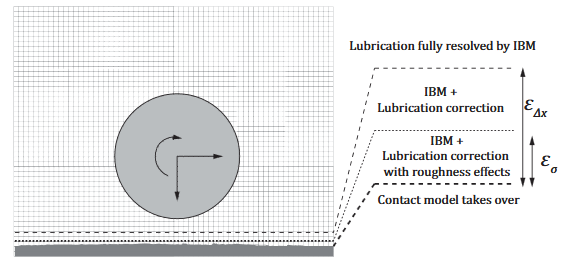
\includegraphics[clip,trim=0 0 0 30,height = 23mm]{IBM.png}\\
	\vspace{-7pt}
	{\hspace{10pt} {\tiny IBM: Costa et al, PRE, 2015}}	
\end{textblock*}
%
\begin{textblock*}{80mm}[0,0](65mm,28mm)
	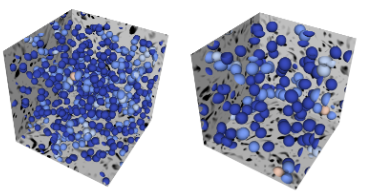
\includegraphics[height = 24mm]{basilisk.png}\\
	\vspace{-12pt}
	{\flushright {\tiny Basilisk: Boniou et al, JFM, 2025}}	
\end{textblock*}
%
\begin{textblock*}{50mm}[0,0](55mm,60mm)
	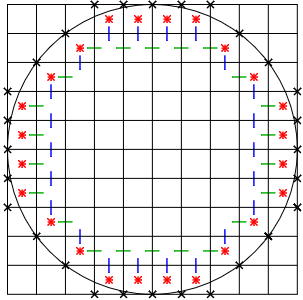
\includegraphics[height = 21mm]{physalis_1.png}
	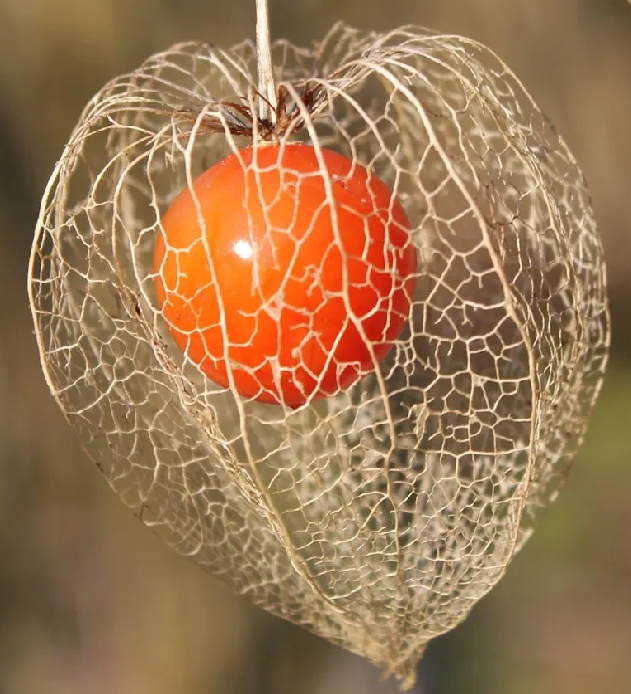
\includegraphics[height = 21mm]{physalis_2.png}\\
	\vspace{-6pt}
	{\tiny Physalis: Naso \& Prosperetti, NJP, 2010}	
\end{textblock*}

}
\frame{
\frametitle{Experiments}
\begin{textblock*}{90mm}[0,0](-8mm,-2mm)
	\textcolor{myred}{\textbf{Turbulent generators}}
\end{textblock*}

\begin{textblock*}{125mm}[0,0](-8mm,2mm)
{\small
\begin{itemize}
\item Wind tunnels:\vspace{-6pt}
	\begin{itemize}
		\item passive or active grids 
		\item \textit{good homogeneity and isotropy}
		\item \textit{strong mean flow}
	\end{itemize}
\item Turbulent boxes:\vspace{-6pt}
	\begin{itemize}
	\item von K\'arm\'an	
	\item polyhedra with fans / motors
	\item oscillating grids
	\item synthetic jets
	\item \textit{vanishing mean low}
	\item \textit{recirculation problem}
	\end{itemize}
\item In situ measurements
\end{itemize}
}
\vspace{4pt}
\only<1>
\small{\textbf{	\textcolor{myred}{Trade off:}}}\vspace{-4pt}
\begin{itemize}
	\item Homogenity and sotropy \vspace{-6pt}
	\item Turbulence level $R_{\lambda}$ \vspace{-6pt}
\end{itemize}
\end{textblock*}
%
%

\begin{textblock*}{80mm}[0,0](65mm,28mm)
	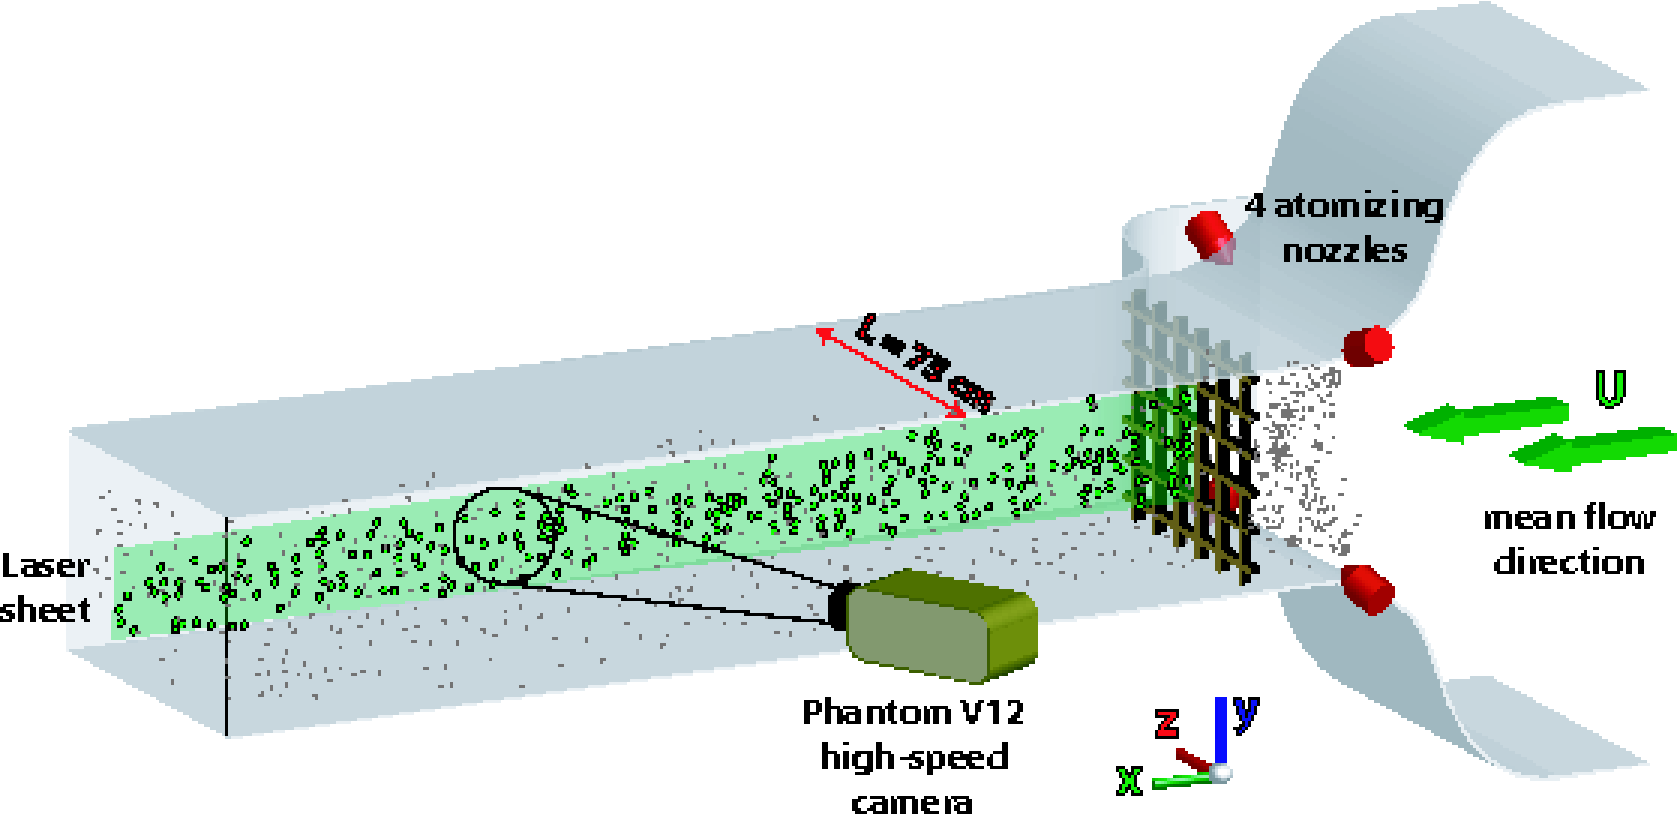
\includegraphics[height = 24mm]{experimentRain.pdf}\\
	\vspace{-12pt}
	{\flushright {\tiny Wind tunnel: Monchaux et al, POF, 2009}}	
\end{textblock*}
%
\begin{textblock*}{38mm}[0,0](54mm,-4mm)
	\flushleft
	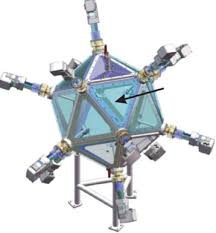
\includegraphics[clip,trim=0 0 0 30,height = 23mm]{LEM.png}\\
	\vspace{-7pt}
	{\hspace{2pt} {\tiny LEM: Zimmerman et al, RSI, 2010}}	
\end{textblock*}
%
\begin{textblock*}{35mm}[0,0](86mm,-4mm)
	\flushleft
	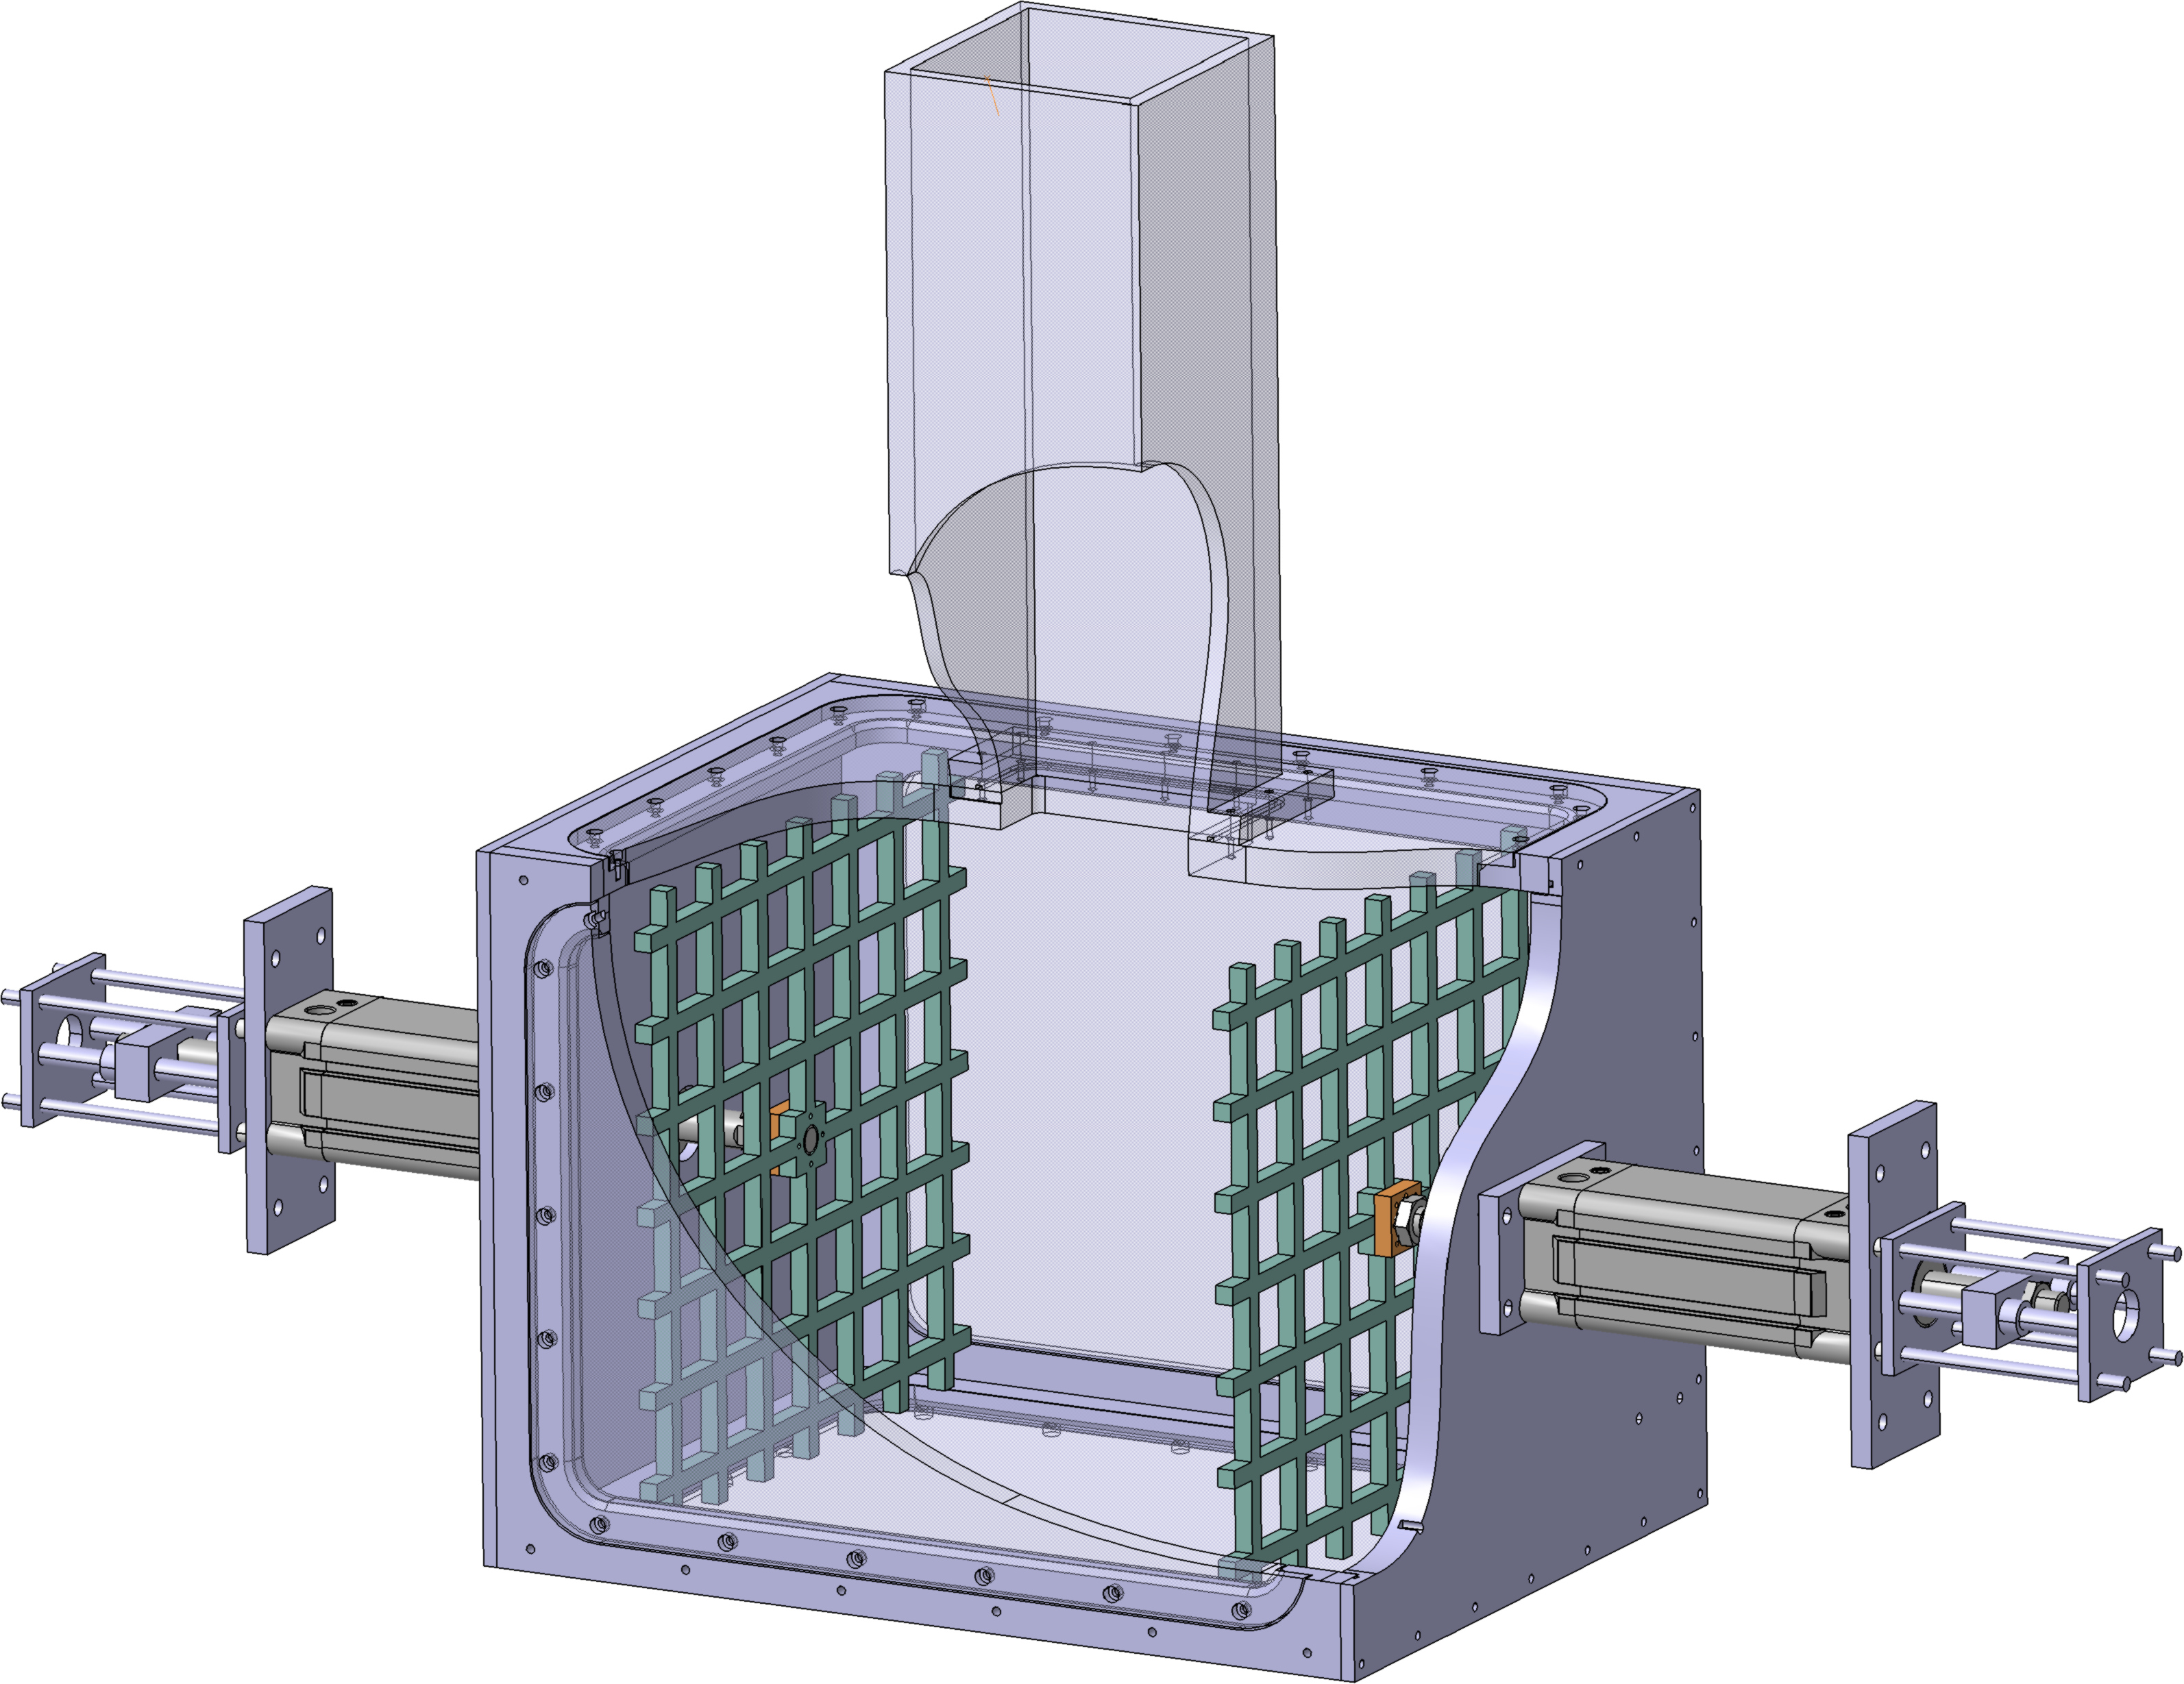
\includegraphics[clip,trim=0 0 0 30,height = 23mm]{Tigrou_isometric_cut2.png}\\
	\vspace{-7pt}
	{\hspace{10pt} {\tiny Oscillating grids: ENSTA}}	
\end{textblock*}
%
\begin{textblock*}{50mm}[0,0](55mm,60mm)
	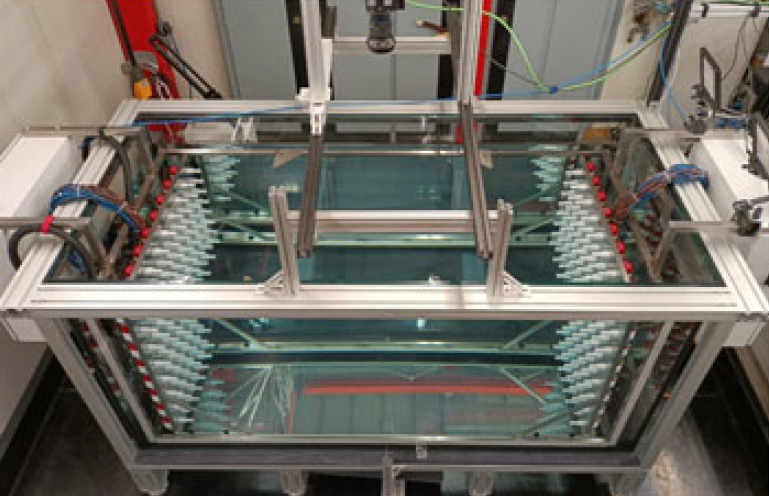
\includegraphics[height = 21mm]{jet_array.png}\\
	\vspace{-6pt}
	{\tiny Jet arrays: Coletti group, Zurich}	
\end{textblock*}

}
\frame{
\frametitle{Experiments}
\begin{textblock*}{90mm}[0,0](-8mm,-2mm)
	\textcolor{myred}{\textbf{Turbulence measurements}}
\end{textblock*}

\begin{textblock*}{125mm}[0,0](-8mm,2mm)
{\small
\begin{itemize}
\item 2D: PIV, PTV\vspace{-4pt}
\item 3D: Tomo-PIV, Holographic PIV, 3D-PTV\vspace{-4pt}
\item Simultaneous fluid+particle:\vspace{-4pt}
\begin{itemize}
	\item fluorescence separation
	\item refractive index matching
	\item scale separation\vspace{-6pt}
\end{itemize} 
\item Opaque flows: \vspace{-4pt}
\begin{itemize}
	\item X-ray PIV
	\item acoustic Doppler
\end{itemize} 

\end{itemize}
}
\vspace{4pt}
\only<1>
\small{\textbf{	\textcolor{myred}{Seeding:}}}\vspace{-4pt}
\begin{itemize}
	\item Particle characterization \vspace{-6pt}
	\item Polydispersity \vspace{-6pt}
	\item Seeding homogeneity \vspace{-6pt}
	\item Disentangling parameters
\end{itemize}
\end{textblock*}
%
%
\begin{textblock*}{80mm}[0,0](65mm,28mm)
	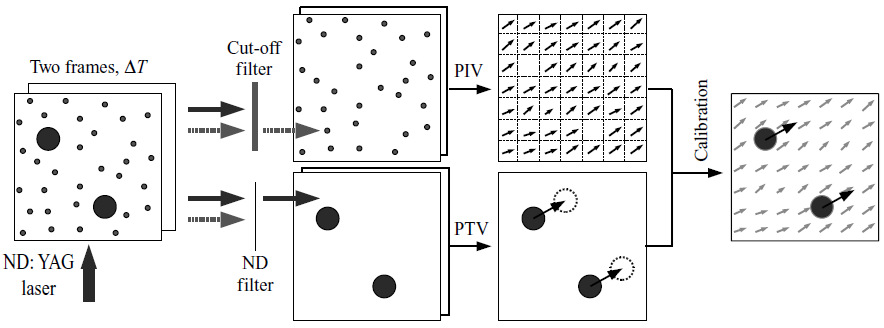
\includegraphics[height = 24mm]{poelma.png}\\
	\vspace{-12pt}
	{\flushright {\tiny Poelma et al, JFM, 2007}}	
\end{textblock*}
%
\begin{textblock*}{80mm}[0,0](70mm,-4mm)
	\flushleft
	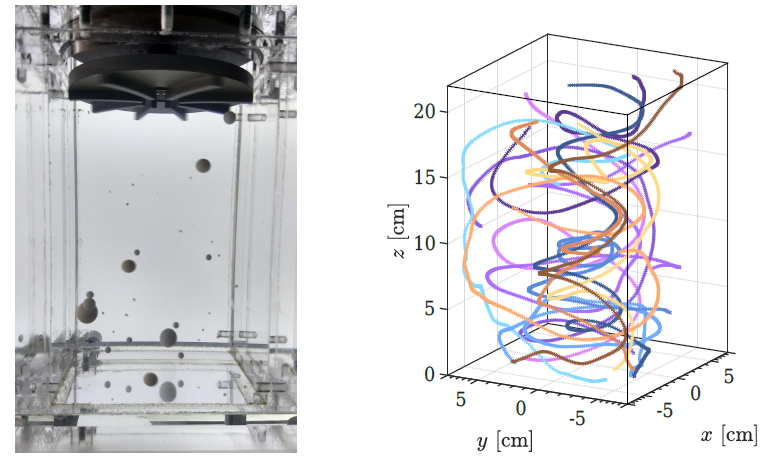
\includegraphics[clip,trim=0 0 0 30,height = 23mm]{laplace.png}\\
	\vspace{-7pt}
	{\hspace{2pt} {\tiny ENS Lyon group}}	
\end{textblock*}
%
\begin{textblock*}{40mm}[0,0](45mm,60mm)
	\includegraphics[height = 21mm]{coletti_PIV1.png}\\
	\vspace{-6pt}
	{\tiny Coletti group, Zurich}	
\end{textblock*}
\begin{textblock*}{50mm}[0,0](96mm,59mm)
	\includegraphics[height = 21mm]{coletti_PIV2.png}
\end{textblock*}

}

%\frame{
\frametitle{Inertial Particles and Turbulence}

\begin{textblock*}{55mm}[0,0](-5mm,0mm)
	\centering
	Density: $\rho_p\neq \rho_f$\\[6pt]
	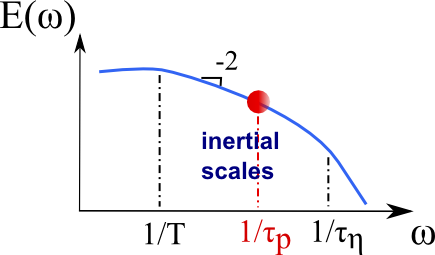
\includegraphics[width=\textwidth]{pseudoSpectre2.png}
\end{textblock*}

\begin{textblock*}{55mm}[0,0](55mm,0mm)
	\centering
	Size: $\eta < D < L$\\[6pt]
	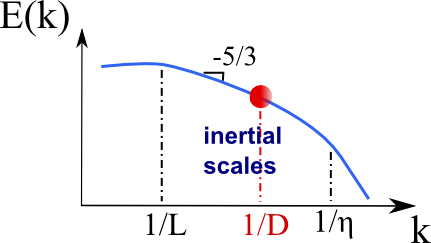
\includegraphics[width=\textwidth]{pseudoSpectre1.png}
\end{textblock*}
%
%
\begin{textblock*}{90mm}[0,0](-5mm,46mm)
	\only<2>{
	\textcolor{myred}{\textbf{Control parameters}}
	}
\end{textblock*}
%
\begin{textblock*}{90mm}[0,0](-10mm,52mm)
	\only<2>{
	\begin{tabular}{ccccc}
		\scriptsize{\textbf{Turbulence}}&
		\scriptsize{\textbf{Inertia}}&
		\scriptsize{\textbf{Gravity}}&
		\scriptsize{\textbf{Gravity}}&
		\scriptsize{\hspace{-2mm}\textbf{Retroaction}}\\[4pt]
		\scriptsize{Reynolds number}&
		\scriptsize{Stokes number}&
		\scriptsize{Rouse number}&
		\scriptsize{Froude number}&
		\scriptsize{Loading}\\
		\footnotesize{$\bold{R_{\lambda}} = \frac{\textcolor{myblue}{u'} \textcolor{myblue}{\lambda}}{\textcolor{myblue}{\nu}};$}&
		\footnotesize{$\bold{St} =  {\frac{2}{9}} \left( \frac{\textcolor{red}{r_p}}{\textcolor{myblue}{\eta}}\right)^2 \left( \frac{\textcolor{red}{\rho_p}}{\textcolor{myblue}{\rho_f}}-1\right);$}&
		\footnotesize{$\bold{R} = \frac{\textcolor{mygreen}{v_t}}{\textcolor{myblue}{u'}}; $}&
		\footnotesize{$\bold{Fr} = \textcolor{myblue}{a_0}^{1/2}\frac{\textcolor{myblue}{\eta} / \textcolor{myblue}{\tau_\eta}^2}{\textcolor{orange}{g}};$}&
		\footnotesize{$\Phi _v$, $\Phi_m$, $n$}
	\end{tabular}
	}
\end{textblock*}


}

%\input{./01_IP_intro/inert_part_intro_00_exemple_04}
%%
%\frame{
\frametitle{Control parameters}
%
\begin{textblock*}{90mm}[0,0](-10mm,0mm)
\begin{tabular}{ccccc}
\scriptsize{Reynolds number}&
\scriptsize{Stokes number}&
\scriptsize{Rouse number}&
\scriptsize{Density ratio}&
\scriptsize{Loading}\\
\footnotesize{$\bold{R_{\lambda}} = \frac{\textcolor{myblue}{u'} \textcolor{myblue}{\lambda}}{\textcolor{myblue}{\nu}};$}&
\footnotesize{$\bold{St} =  \tiny{\frac{2}{9}} \left( \frac{\textcolor{red}{r_p}}{\textcolor{myblue}{\eta}}\right)^2 \left( \frac{\textcolor{red}{\rho_p}}{\textcolor{myblue}{\rho_f}}-1\right);$}&
\footnotesize{$\bold{R} = \frac{\textcolor{mygreen}{v_t}}{\textcolor{myblue}{u'}}; $}&
\footnotesize{${\Gamma} = \frac{\textcolor{red}{\rho _p} }{\textcolor{myblue}{\rho _f}};$}&
%\footnotesize{$\bold{Gamma} = \frac{\textcolor{red}{\rho _p}}/ \textcolor{myblue}{\rho _f}};$}&
\footnotesize{${\Phi _v}.$}\\[8pt]
\scriptsize{\textbf{Turbulence}}&
\scriptsize{\textbf{Inertia}}&
\scriptsize{\textbf{Gravity}}&
\scriptsize{\textbf{Density}}&
\scriptsize{\hspace{-2mm}\textbf{Retroaction}}\\[8pt]
\scriptsize{$10-10^4$}&
\scriptsize{$10^{-5}-10^2$}&
\scriptsize{$0-10$}&
\scriptsize{$10^{-4}-10^3$}&
\scriptsize{\hspace{-3mm}$10^{-6}-10^{-1}$}
\end{tabular}
\end{textblock*}
%\scriptsize{}&
%

\begin{textblock*}{75mm}[0,0](40mm,25mm)
\onslide*<2->{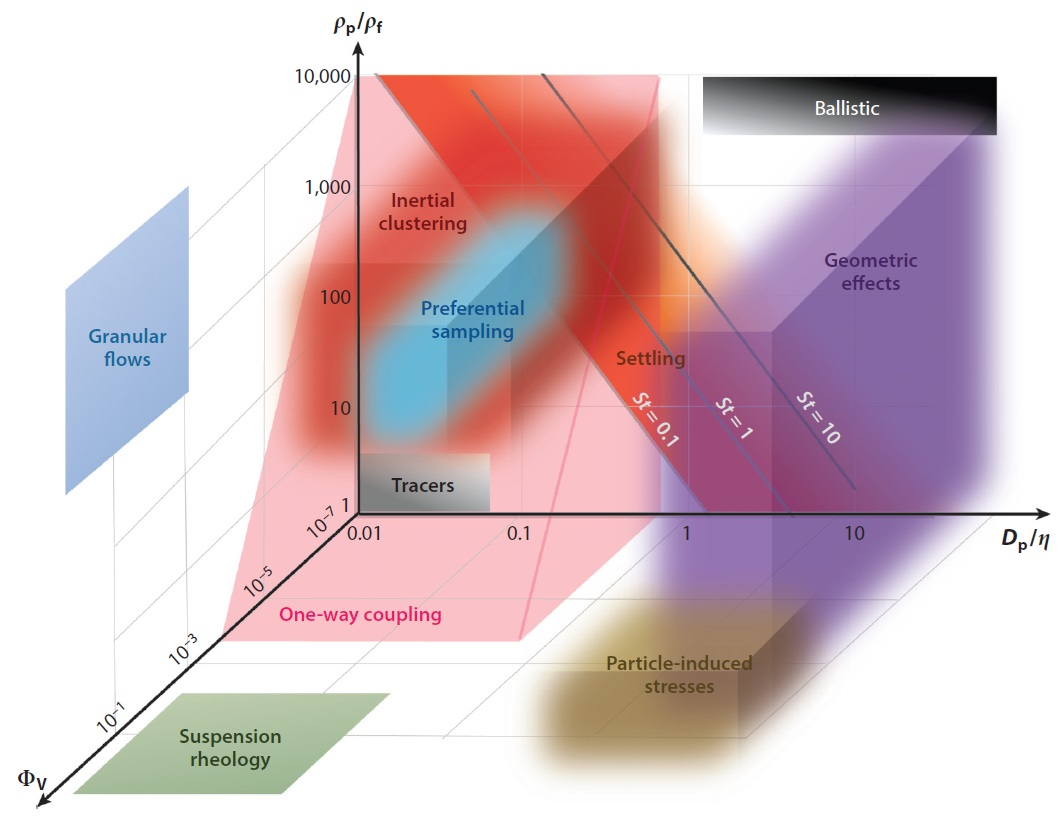
\includegraphics[width = \textwidth]{phase_space_colletti.jpg}}
\end{textblock*}
\begin{textblock*}{20mm}[0,0](95mm,73mm)
{\tiny
\begin{flushright}
\onslide*<2->{	Brandt \& Coletti, \textit{Annual Review}, \textbf{2022}}
\end{flushright}
}
\end{textblock*}
%

\begin{textblock*}{90mm}[0,0](-5mm,32mm)
	{\footnotesize
		\begin{itemize}
			\item Particle Reynolds number
			\item Galileo number
			\item Aspect ratio
			\item Deformability
			\item \ldots
	\end{itemize}}
\end{textblock*}

\begin{textblock*}{50mm}[0,0](-5mm,62mm)
\onslide*<3>{
{\small 
\textcolor{myred}{
\textbf{
Intertwined parameters\\[3pt]}
$\implies$ complementary simulations and experiments}
}}
\end{textblock*}
%
%
}



%\input{./01_IP_intro/inert_part_intro_03_tools_01}
%\input{./01_IP_intro/inert_part_intro_03_tools_02}
%%
%\input{./01_IP_intro/inert_part_intro_06_PC_01}
%\input{./01_IP_intro/inert_part_intro_06_PC_02}
%\input{./01_IP_intro/inert_part_intro_06_Sett_01}
%%\input{./01_IP_intro/inert_part_intro_06_Sett_02}
%
%
%\section{Results - Preferential concentration}
%\input{./02_IP_results/inert_part_results_setups_01}
%\input{./02_IP_results/inert_part_results_setups_02}
%%%
%\input{./02_IP_results/inert_part_results_PC_voro_01}
%\input{./02_IP_results/inert_part_results_PC_voro_02}
%\input{./02_IP_results/inert_part_results_PC_voro_03}
%%\input{./02_IP_results/inert_part_results_PC_voro_04}
%%\input{./02_IP_results/inert_part_results_PC_voro_05}
%%
%\input{./02_IP_results/inert_part_results_PC_cluster_01}
%\input{./02_IP_results/inert_part_results_PC_cluster_02}
%\input{./02_IP_results/inert_part_results_PC_cluster_03}
%\input{./02_IP_results/inert_part_results_PC_cluster_04}
%
%\section{Results - Settling alteration}
%\input{./02_IP_results/inert_part_results_Sett_01}
%\input{./02_IP_results/inert_part_results_Sett_02}
%\input{./02_IP_results/inert_part_results_Sett_03}
%%%
%\section{Results - Tigrou}
%\input{./03_Tigrou/tigrou_param_02}
%\input{./03_Tigrou/tigrou_results_Vset_01}
%\input{./03_Tigrou/tigrou_results_Voro_01}
%\input{./03_Tigrou/double_mes_01}

%\addtocounter{framenumber}{-3}%
%
\end{document}
